\documentclass[conference]{IEEEtran}
\IEEEoverridecommandlockouts
% The preceding line is only needed to identify funding in the first footnote. If that is unneeded, please comment it out.
\usepackage{listings}
\usepackage{cite}
\usepackage{amsmath,amssymb,amsfonts}
\usepackage{algorithmic}
\usepackage{graphicx}
\usepackage{textcomp}
\usepackage{xcolor}
\usepackage{hyperref}
\usepackage{cleveref}
\usepackage{dirtytalk}
\usepackage{verbatim}

\usepackage[outputdir=build]{minted}
% \usemintedstyle{default}
% \setminted{frame=single}
% \setminted{framesep=2mm}
% \setminted{fontsize=\footnotesize}

\usepackage[T1]{fontenc}
\renewcommand{\ttdefault}{cmtt}

\begin{document}

\title{Networked Embedded Systems Practical Project}

\author{\IEEEauthorblockN{Siyan Chen}
\IEEEauthorblockA{\textit{Technical University of Denmark} \\
siyan@chen.com}
\and
\IEEEauthorblockN{Evangelos Lamprou}
\IEEEauthorblockA{\textit{Technical University of Denmark} \\
e.lamprou@upnet.gr}
}

\maketitle

\begin{abstract}
    In this project, we present creation of an
    embedded network system using the popular ESP32 platform. The system serves
    the purpose of recording audio samples and facilitating their remote
    transmission over the Internet. We go into the design and implementation
    of the sytem while simultaneously putting attention
    on pivotal security considerations that touch multiple
    layers of the architecture. 
\end{abstract}

\begin{IEEEkeywords}
embedded network systems, security
\end{IEEEkeywords}

\section{Introduction}

Embedded network systems have burgeoned as critical assets across numerous
domains, encompassing home automation, industrial monitoring, and beyond. 
The proliferation of the Internet of Things (IoT) has further accelerated the
adoption of such systems\cite{IotTechEmbedded}.
However, their security has been a major concern,\cite{EmbeddedSecSurveyEU}
as their widespread use has made them a target for malicious actors, 
with the platforms themselves being vulnerable because of their low computational power and
rapid development cycles\cite{EmbeddedSecChallenges}.
In this work, we aim to provide a set of security solutions that do not employ 
heavy cryptographic primitives or complex remote attestation protocols, but rather
focus on the use of simple and lightweight techniques that can be easily implemented
on resource-constrained devices.

This report is structured as follows: in \cref{sec:background}, 
we give a short overview of our project's goals while providing references to similar works. 
In \cref{sec:system_design}, we go into the design of the system, giving a high-level overview of the architecture and 
the components used. Then, in \cref{sec:system_implementation}, we go over the final implementation and comment on it's performance, 
while also highligthing some of the security considerations we took into account. Finally, in \cref{sec:discussion_and_conclusions},
we discuss the results of our work and propose some ideas for future work.

\section{Project Objectives} % Project Objectives 
\label{sec:background}

The goal of this project is to create a networked embedded system that can record audio samples and transmit them over the Internet.
The use case could be a remote monitoring system, where the device is placed in a remote location and 
the user can listen to an audio feed from their device. Applications such as baby monitors or home security systems come to mind.
In both of these cases, the confidentiality of the audio feed is very important and
attacks on such systems have been demonstrated in the past \cite{BabyMonitorHack, VideoSurvAttacks}.

\section{System Design}
\label{sec:system_design}

\subsection{Architecture}

\begin{figure}[h]
    \hspace*{-0.4cm}
    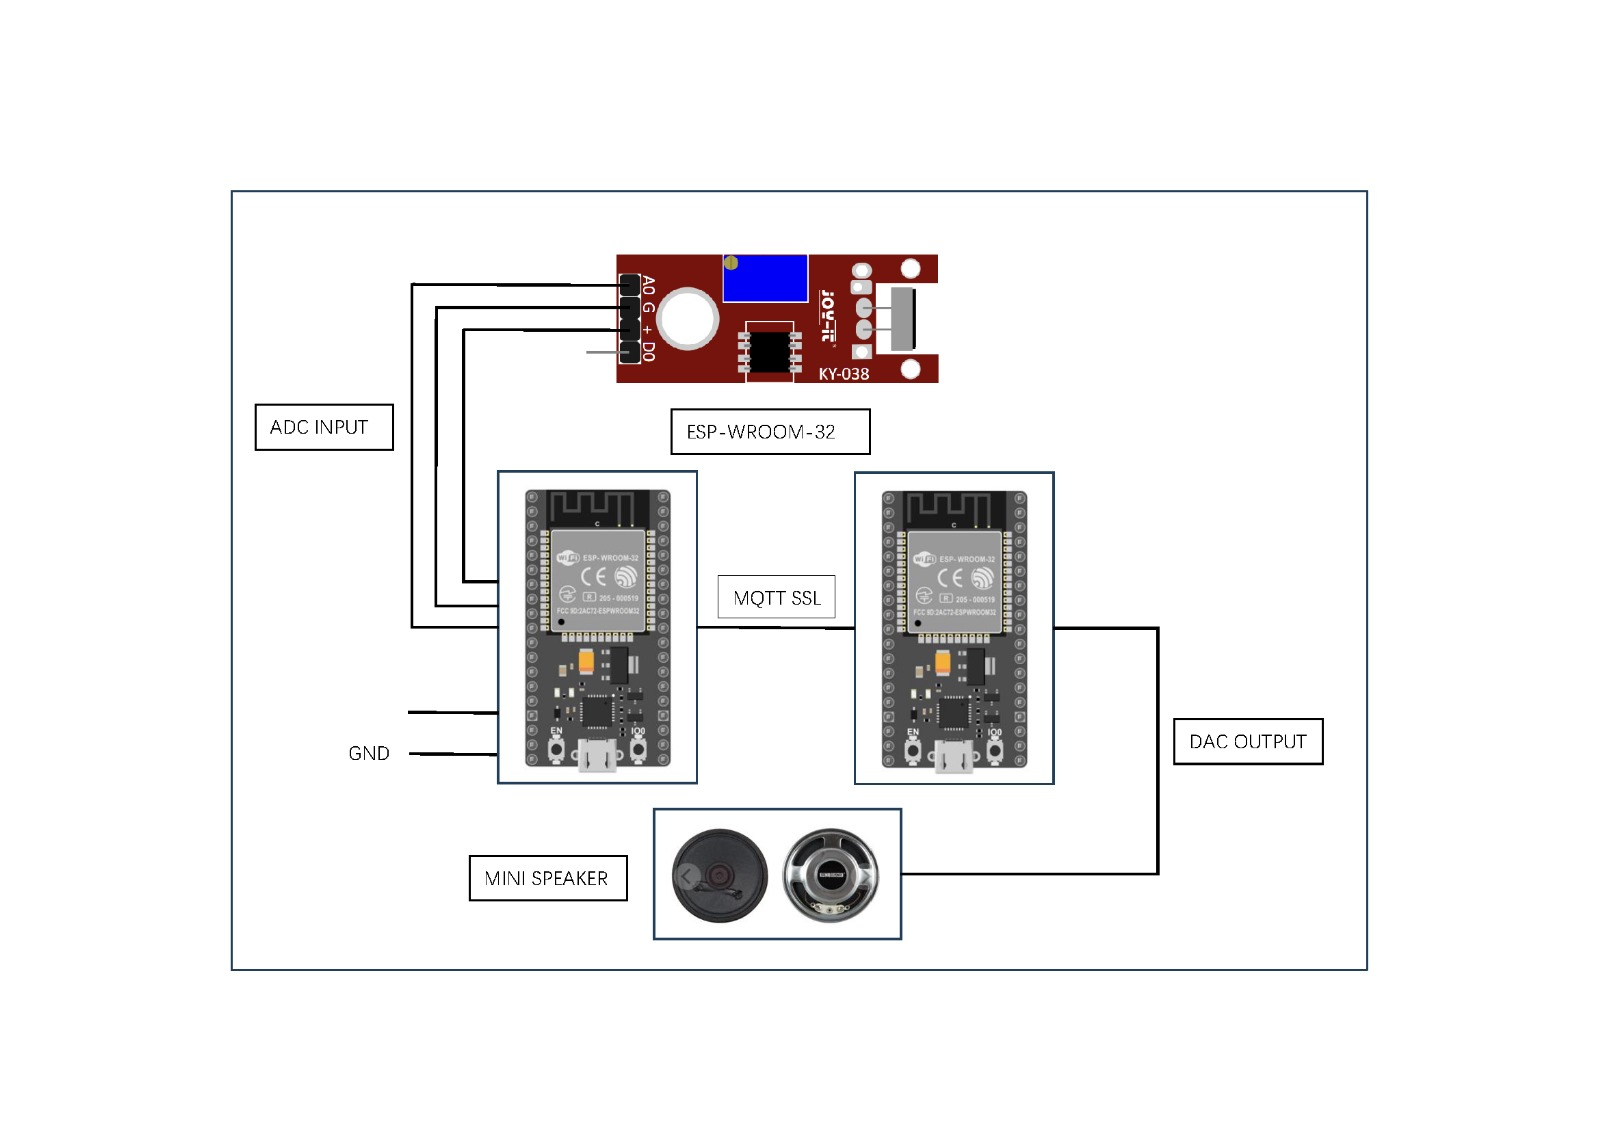
\includegraphics[width=1.2\linewidth]{assets/diagram.png}
    \vspace{-1.5cm}
    \caption{High-level overview of the system architecture.}
    \label{fig:architecture}
\end{figure}

\subsection{Hardware Setup}
The system consists of two ESP32\cite{ESP32_Manual} microcontrollers.
As an input device, we use the KY-038\cite{KY-038} microphone sound sensor.
The sensor allows for both digital and analog output, with the digital output being a simple
on/off signal and the analog output being a voltage signal that is proportional to the sound intensity.
For our purposes, we use the analog output, converting the voltage signal to a digital one using the
ESP32's analog-to-digital converter (ADC).
For the receiver device, we used a simple mini-speaker that is connected to the ESP32's digital-to-analog converter (DAC).

\subsection{Software and Firmware}

For programming the ESP32 devices, we used the Espressif Systems' ESP-IDF\cite{ESP-IDF}
software development environment. The SDE is written in the C programming 
language. For cross-compiling our source code to the ESP platform we used the \texttt{GCC}-based
\texttt{xtensa-esp32-elf} compiler. 
For the operating system, we used the FreeRTOS\cite{FreeRTOS} real-time operating system
in order to take advantage of the provided task management features.
\subsection{Communcation}

Communication between the two devices is done using the Message Queuing Telemetry Transport (MQTT) protocol\cite{MQTT_Survey}.
MQTT is a lightweight publish/subscribe messaging protocol that is designed for constrained devices and low-bandwidth.
A publisher sends a message to the broker, which then forwards the message to all the subscribers that are subscribed to a given topics.
Topics are strings used to identify the messages and are organized in a hierarchical structure.
We used MQTT because of it's simple programming model, as most of the communication logic is handled by the broker.
For our project, we used a free public broker\footnote{hiveMQ: \url{https://www.hivemq.com/public-mqtt-broker/}}.

\section{System Implementation}
\label{sec:system_implementation}

\subsection{Firmware and Hardware}

The firmware for the two devices is written in C and is structured in a modular way.
The main program logic is separated into two files, one for the recording device and one for the playback device.
The recording device is responsible for recording audio samples and sending them to the server.
The playback device is responsible for receiving the audio samples from the server and playing them back.

The FreeRTOS provided API allows us to easily create parallel tasks that are then scheduled by the operating system.
We have a listening task and a action task for each of the devices.
For the recording device, a task is responsible for recording audio samples and saving them 
inside a circular buffer data structure. Asyncronously, a second task is responsible for
sending the samples to the server using the MQTT protocol.
For the playback device, a task is responsible for receiving the samples from the server
and another one for playback.

One challenge we encoutered was choosing the correct stack size for each created thread.
We wanted to use the minimum stack size possible.
For that, we used the FreeRTOS \texttt{uxTaskGetStackHighWaterMark} function, which returns
the available stack space for a given thread.
We set our stack size to the size allocated minus the value returned by the function plus a safety margin.
A more robust solution would also include a code coverage analysis\cite{CodeCoverage} of the program,
making sure that there are no code paths where the stack overflows.



\subsection{Security Analysis}
\label{subsec:security_analysis}


\subsubsection{Threat Model}

We assume a strong software adversary that has physical access to the device.
A persistent attacker might be able to extract the firmware from the device and
analyze it. Such analysis can result in cryptographic keys and certificates being extracted from the device
\footnote{In \cref{appendix:reverse_engineering} we provide a tutorial-like section where we act as an attacker and attempt to reverse engineer the firmware of an ESP32 device.}, 
to the proprietary program logic being reverse engineered.
In addition, the device might be placed in an untrusted environment, where the communication as well 
as other networking infrastructure might tampered with.
An adversary might be able to \say{listen} to the communication between the two devices,
as they might be inside the same network.
Thus, the adversary might be able to perform a wide range of network attacks such 
as a DNS Cache Poisoning attack \cite{Dissanayake_2018}, the adversary might have access to the local router 
settings, making a Domain Hijacking and Redirection attack \cite{DnsHijacking} trivial. In both of these attacks, 
the data transferred from the recording device to the server might be redirected to a malicious server, 
where the data might be stored and analyzed.

\subsubsection{Security Considerations}

\paragraph{Communication}

In order to make communication between the two devices and the MQTT broker
trusted, we initiate an SSL (Secure Socket Layer) connection to the public broker. 
The use of SSL/TLS (Transport Layer Security)
ensures the confidentiality and integrity of data transmission. 
It achieves this by encrypting the data in transit, preventing
unauthorized access and eavesdropping. The SSL connection also provides a means
to verify the authenticity of the MQTT broker.
The use of certificates, and thus asymmetric encryption might be inappropriate in the scenario where more 
memory constrained devices are part of the network. 
An alternative is the use of Transport Layer Security pre-shared key (TLS-PSK)\cite{rfc4279}, where the two parties 
(device and broker) have a common key which they use to encrypt their communication channel.
However, this approach requires the establishment of a key exchange routine before communication can start
and creates protocol complexity.

\paragraph{Message Encryption}

Even if the communication between the two parties is (apparently) secured, data still needs to be encrypted because of the possibility 
of the communication channel being compromised (e.g through a Wi-Fi spoofing attack \cite{WifiSpoofing}, where an attacker 
impersonates a Wi-Fi access point by using the same SSID) or the data being stored inside a server.
For message encryption, we use the Advanced Encryption Standard (AES) on cipher feedback (CFB) mode using 
a common 32-byte pre-shared key between the two devices.
The ESP32 offers hardware accelerated AES encryption and decryption routines\footnote{The ESP-IDF implementation of the AES routine can be found in \texttt{components/mbedtls/port/aes/block/esp\_aes.c},
with some attacks on the implementation being presented in \cite{PwnEsp32Crypto}.}.

In our implementation, the key is stored inside the program's source code using 
a simple obsfucation function that shuffles the keys deterministically before using it, essentially
making it so the key can not be \textit{easily} obtained from static inspection of the firmeware.
Other alternatives would be to use a key exchange protocol such as Diffie-Hellman key exchange\cite{DiffieHellmanKeyExchange} to 
establish a common key between the two devices or store the key in one of ESP32's eFuse blocks.
Each audio sample (a byte buffer of variable size) is encrypted using the key 
and subsequently sent.

\paragraph{Program Logic}

To avoid the possibility of buffer overflow attacks, where a malicious user might be able 
to write to memory locations outside designated areas (such as outside the circular buffer that saves
the audio samples) we enable the \texttt{CHECK\_FOR\_STACK\_OVERFLOW} option in the FreeRTOS configuration.
This way, the kernel will check that the stack pointer register is within the stack bounds on every context switch.
In addition, we added our own assertions in places where buffer overflows might occur.

In order to avoid the possibility of extracting the firmware from the device,
we enabled the flash encryption feature. This is done by enabling the
correspoding eFuse bit\footnote{eFuse bits are one-time programmable bits that
can be used to store system and user parameters. Thus, it is recommended to
modify them at the latest possible stage of the development process.}. While
there exist other more involved hardware-based reverse engineering
countermeasures \cite{HardwareReverseEngineering}, we used one that the ESP32
provides out-of-the-box.
A software-oriented approach in order to mitigate the possibility of someone reverse-engineering the firmware would be to use
a virtual machine-based approach\footnote{An popular project for virtualizing the x86 architecure can be found at \url{https://github.com/rwfpl/rewolf-x86-virtualizer}},
where the firmware is run inside a virtual machine that is hosted on the device.
Using this approach, reverse engineering tools that rely on analysis of
assembly instructions would not be able to accurately recreate the program
code.
% In our project, we tried to employ the \textit{Elk}\cite{Elk} lightweight javascript virtual machine
% to implement the sample storing logic, but removed it in the final version due to time constraints.


\section{Discussion and Conclusions}
\label{sec:discussion_and_conclusions}

In this project, we have presented the design and implementation of a networked embedded system
that can record audio samples and transmit them over the Internet.
We touched upon some of the security considerations that need to be taken into account when designing such a system.
In particular, we:

\begin{itemize}
    \item Utilized secure communication protocols to ensure the confidentiality and integrity of the data transmission.
    \item Used SSL/TLS to secure the communication channel between the two devices and the MQTT broker.
    \item Used AES encryption to encrypt the audio samples before sending them over the network.
    \item Used FreeRTOS's stack overflow checking feature to avoid buffer overflow attacks.
    \item Used a simple obsfucation function to hide the encryption key from static inspection of the firmware.
    \item Enabled ESP32's flash encryption feature to avoid the possibility of extracting the firmware from the device.
\end{itemize}

\section*{Acknowledgment}

\thanks{We'd like to thank the DTU PRG group for providing us with some of the hardware and equipment for this project.}

\bibliographystyle{IEEEtran}
\bibliography{IEEEabrv,bibliography}

\appendices
\crefalias{section}{appendix}

\appendix{Reverse Engineering ESP32 Firmware}
\label{appendix:reverse_engineering}

As proof of the necessity for taking precautions when shipping an embedded device, 
we provide a tutorial-like section where we act as an attacker and attempt to reverse engineer the firmware of an ESP32
device in order to extract sensitive information.

\begin{listing}[h]
\begin{verbatim}
$ esptool.py read_flash $START $END flash.bin
$ ./esp32_image_parser.py show_partitions flash.bin
$ ./esp32_image_parser.py create_elf flash.bin\
                            -partition ota_1\
                            -output ota_1.elf
\end{verbatim}
\caption{The sequence commands for extracting the flash contents and converting them to an ELF file.}
\end{listing}

After gettings the device's firmeware into ELF format, we can use a plethora of tools 
to reverse engineer the underlying program. 
In this example, we will conduct a static analysis of the binary using the popular Ghidra\cite{Ghidra,GhidraBook} analysis tool.
We use the \texttt{ghidra-xtensa}\footnote{\url{https://github.com/yath/ghidra-xtensa}} processor,
which adds support for the Xtensa architecture, the architecture used by the ESP32.

\begin{figure}[h]
    \centering
    \fbox{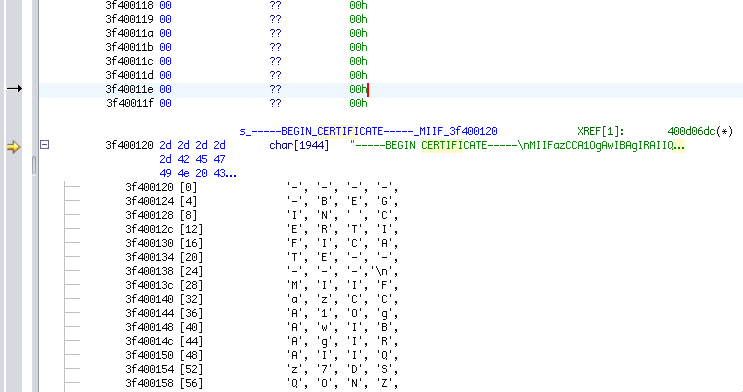
\includegraphics[width=.9\linewidth]{assets/ghidra.png}}
    \caption{Screeshot inside Ghidra where we are able to read the used certificate. Simmilalry, 
    by inspecting the \texttt{rodata} flash section we can find the broker domain the device is conncectiing to, the 
    symmetric encryption key used for message encryption.}
    \label{fig:ghidra}
\end{figure}

An attacker can further attack the device by performing dynamic analysis using the \texttt{qemu-xtensa} emulator
by plugging to it the \texttt{gdb} debugger. 
Using those tools, we can follow the program execution and extract the symmetric encryption key used for message encryption, 
even is that key is not stored in the flash memory, but is generated at runtime.

\end{document}
